% =============================================================================
% Capitulo 1 - Introduccion
% =============================================================================
\chapter{Introducción}
\label{cap:introduccion}

\section{Contexto y motivación}
\label{sec:contexto}

El uso de vehículos aéreos no tripulados, habitualmente denominados drones o UAV (\emph{Unmanned Aerial Vehicles}), ha aumentado de forma notable durante los últimos años. Su bajo coste, su facilidad de manejo y la disponibilidad de sistemas comerciales con cámara, estabilización y enlaces digitales de control y vídeo han facilitado su empleo en fotografía, inspección, ocio, agricultura de precisión y vigilancia. Sin embargo, esta misma expansión también plantea problemas de seguridad y privacidad cuando los drones operan en zonas no autorizadas, cerca de infraestructuras críticas, aeropuertos, eventos multitudinarios o espacios urbanos sensibles.

Existen diferentes aproximaciones para la detección de drones: sistemas ópticos, acústicos, radar y sistemas basados en radiofrecuencia. Cada familia presenta ventajas y limitaciones. Las cámaras pueden verse afectadas por iluminación, obstáculos o condiciones meteorológicas; los sensores acústicos sufren en entornos ruidosos; y los radares de altas prestaciones pueden resultar costosos para escenarios de bajo presupuesto. Frente a ello, la detección mediante radiofrecuencia resulta especialmente interesante porque muchos drones comerciales mantienen un enlace activo con el mando de control o con el dispositivo móvil del operador. Detectar dicho enlace permite inferir actividad de dron incluso cuando el vehículo no es claramente visible.


El presente trabajo se centra en la banda ISM de \SI{2.4}{\giga\hertz}, una de las bandas más utilizadas por sistemas inalámbricos comerciales. Esta elección introduce una dificultad práctica importante: la señal del dron debe analizarse en un entorno compartido con múltiples transmisiones, especialmente redes WiFi y dispositivos Bluetooth. Por tanto, el problema no consiste únicamente en detectar un aumento de potencia en el espectro, sino en distinguir si la morfología tiempo-frecuencia observada corresponde a un enlace de dron o a interferencias habituales de la banda.

En particular, se estudia el caso de un dron DJI Mini 3. Su enlace de comunicaciones OcuSync O2 genera ráfagas de transmisión observables en el dominio tiempo-frecuencia. Estas ráfagas aparecen en los espectrogramas como estructuras estrechas y de corta duración, distribuidas a lo largo de la banda analizada. Sin embargo, otras tecnologías presentes en \SI{2.4}{\giga\hertz}, especialmente Bluetooth, también emplean mecanismos de salto en frecuencia y pueden producir patrones parcialmente similares. Esta similitud convierte el problema en una tarea de análisis morfológico de ráfagas FHSS, no en una simple separación por potencia.

\begin{figure}[htbp]
    \centering
    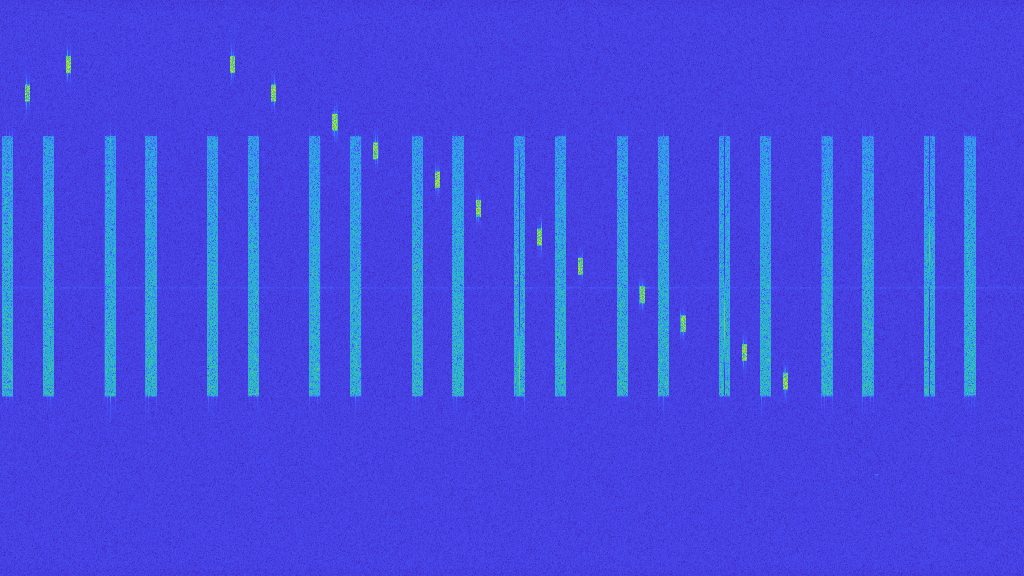
\includegraphics[width=0.90\textwidth]{figuras/introduccion/mini3_drone_d5_w1_s01_cap01__seg0028.png}
    \caption{Ejemplo de espectrograma obtenido a partir de una captura RF del DJI Mini 3 en la banda de \SI{2.4}{\giga\hertz}. Se observan ráfagas estrechas y de corta duración distribuidas en frecuencia, correspondientes a la firma tiempo-frecuencia característica del enlace de comunicaciones del dron. Las bandas más anchas y prolongadas en el tiempo se corresponden con el enlace de descarga de vídeo (\emph{downlink}) del dron, mientras que las ráfagas más estrechas se asocian al canal de control.}
    \label{fig:espectrograma_mini3}
\end{figure}

La formulación inicial del trabajo planteaba una clasificación binaria de espectrogramas completos mediante una red convolucional ResNet18. Aunque este enfoque permitía construir un primer prototipo, el análisis experimental mostró una limitación importante: un clasificador global puede aprender correlaciones espurias del contexto de captura, como diferencias entre escenarios interiores y exteriores, en lugar de centrarse en la firma RF local del dron. Para evitar este problema, el trabajo se reconvierte hacia un detector de objetos basado en YOLOv8 que opera sobre regiones del espectrograma. De este modo, el modelo debe localizar y clasificar ráfagas individuales, reduciendo la dependencia del fondo global de la imagen.

Este cambio conecta el trabajo con arquitecturas recientes de detección e identificación RF en dos etapas, donde una primera red detecta regiones de señal en el espectrograma y una segunda red clasifica el tipo de dron a partir de las regiones detectadas \cite{rfuav2025}. En este TFG, la primera etapa se centra en separar ráfagas asociadas al DJI Mini 3 frente a interferencias WiFi/Bluetooth, y la segunda etapa identifica el modelo concreto de dron a partir de esas regiones, una vez confirmada la presencia de señal.

\section{Planteamiento del problema}
\label{sec:planteamiento}

El problema principal abordado se formula como una tarea de detección de objetos sobre espectrogramas RF. Dada una ventana temporal de señal capturada mediante un receptor SDR, se desea localizar las regiones del espectrograma que contienen ráfagas de señal y clasificarlas como \emph{drone} o \emph{interference}. La clase \emph{drone} representa ráfagas compatibles con la firma OcuSync del DJI Mini 3, mientras que la clase \emph{interference} agrupa ráfagas y estructuras producidas por fuentes no dron, principalmente Bluetooth FHSS, WiFi residual y ruido que supera el umbral de etiquetado.

La dificultad reside en que la banda analizada está compartida por múltiples tecnologías inalámbricas. Una simple medida de potencia recibida no resulta suficiente, ya que una red WiFi cercana puede generar niveles de energía elevados y producir falsas alarmas si el sistema se basa únicamente en umbrales. Además, algunas señales interferentes, como Bluetooth, presentan ráfagas estrechas y saltos en frecuencia que pueden asemejarse parcialmente a la firma del enlace del dron. Por este motivo, el detector se plantea sobre espectrogramas, donde se conserva la evolución temporal y frecuencial de la señal.

La hipótesis de trabajo es que la firma FHSS/OcuSync del DJI Mini 3 deja una huella tiempo-frecuencia diferenciable respecto a otras transmisiones presentes en el entorno, y que un detector de objetos puede aprender dicha huella a partir de cajas generadas sobre las regiones activas del espectrograma. A diferencia de la clasificación de imagen completa, la detección de objetos obliga al modelo a operar sobre regiones locales y permite obtener una salida más interpretable: no solo indica si hay dron, sino también dónde aparece la evidencia dentro de la representación tiempo-frecuencia.

Este planteamiento en dos etapas admite una lectura orientada a producto. La primera etapa actúa como un filtro que permite descartar, a modo de lista blanca, las emisiones no relevantes de la banda —WiFi, Bluetooth y ruido residual—, de modo que el sistema solo retiene las regiones compatibles con un enlace de dron. La segunda etapa opera sobre esas regiones ya filtradas y se orienta a la identificación entre diferentes modelos de dron. Esta tarea plantea una dificultad adicional, ya que no basta con distinguir la presencia de una señal compatible con un UAV frente a interferencias, sino que es necesario identificar diferencias más sutiles entre las firmas RF de distintos enlaces de comunicación. Por ello, dicha clasificación se aplica preferentemente sobre las regiones ya detectadas como señal de dron, y no sobre el espectrograma completo.

De forma complementaria, el trabajo evalúa la robustez del sistema frente a la congestión de la banda y frente al ruido, así como su capacidad de generalizar a otros modelos de dron no vistos durante el entrenamiento. El efecto de la distancia entre dron y receptor se contempla únicamente como variable experimental de las capturas ---a 5 y 10 metros---, sin abordarse como un estudio sistemático ni como un problema de localización métrica; su análisis en profundidad se deja como línea futura.

\section{Objetivos}
\label{sec:objetivos}

\subsection{Objetivo general}

El objetivo principal de este Trabajo Fin de Grado es diseñar, implementar y evaluar un sistema de detección de señales de dron mediante radiofrecuencia, utilizando capturas SDR, espectrogramas tiempo-frecuencia y redes neuronales profundas. El sistema se reformula como una arquitectura en dos etapas: una primera etapa de detección/localización de ráfagas mediante YOLOv8 para distinguir \emph{drone} frente a \emph{interference}, y una segunda etapa de identificación de modelos de dron a partir de señales ya detectadas como compatibles con UAV.

\subsection{Objetivos específicos}

\begin{description}
  \item[OE1] Revisar el estado del arte en detección de drones por radiofrecuencia, prestando especial atención a las técnicas basadas en espectrogramas, detección de objetos y arquitecturas en dos etapas.
  \item[OE2] Definir la metodología de adquisición de señales IQ con SDR en la banda de \SI{2.4}{\giga\hertz} (dron activo e interferencias WiFi/Bluetooth bajo condiciones controladas) y construir un conjunto de datos reproducible a partir de capturas SigMF: segmentación en ventanas de \SI{0.1}{\second}, generación de espectrogramas y auto-etiquetado de cajas delimitadoras mediante umbrales de energía y filtros morfológicos.
  \item[OE3] Entrenar y evaluar un detector YOLOv8 que localice y clasifique las ráfagas como \emph{drone} o \emph{interference}, utilizando métricas propias de detección (precisión, recall, mAP@50 y mAP@50-95), y compararlo con el enfoque previo de clasificación global para justificar la reducción del sesgo contextual.
  \item[OE4] Analizar la robustez del sistema frente a la congestión de la banda (WiFi y Bluetooth) y frente al ruido, verificando si la discriminación aprendida se sustenta en la morfología espectro-temporal de las ráfagas o en el nivel medio de potencia.
  \item[OE5] Desarrollar y evaluar una segunda etapa de identificación entre modelos de dron, basada en redes convolucionales como ResNet18, aplicada sobre las regiones o espectrogramas filtrados por la etapa de detección, y comprobar su capacidad de generalización a drones no vistos en el entrenamiento.
\end{description}

\section{Alcance del trabajo}
\label{sec:alcance}

El alcance principal del TFG queda delimitado a la detección de actividad de dron frente a interferencias en espectrogramas RF de la banda de \SI{2.4}{\giga\hertz}. El sistema se valida con capturas reales del DJI Mini 3 y escenarios sin dron con presencia de WiFi/Bluetooth. La contribución central no es decodificar protocolos propietarios ni estimar la posición exacta del dron, sino evaluar si la morfología tiempo-frecuencia de las ráfagas permite distinguir señal de dron frente a interferencias mediante aprendizaje profundo.

El trabajo incluye la adquisición de señales IQ, su almacenamiento en formato SigMF, la generación de espectrogramas, el auto-etiquetado de regiones activas, el entrenamiento de un detector YOLOv8 y la evaluación del modelo con métricas de detección. La identificación de modelos de drones constituye la segunda etapa del sistema, aplicada sobre las regiones filtradas por la detección inicial. La distancia entre dron y receptor se contempla solo como variable experimental de las capturas, no como un sistema de localización ni como un estudio sistemático de su efecto.

Cabe plantearse si este problema podría resolverse analizando directamente los paquetes de datos transmitidos en la banda ISM, en lugar de su morfología tiempo-frecuencia. Sin embargo, este enfoque no es viable en el caso general: los enlaces de comunicación de los drones comerciales, como OcuSync de DJI, emplean protocolos propietarios y cifrado de la información, por lo que el contenido de los paquetes no resulta accesible ni decodificable por un receptor pasivo. El análisis basado en la firma RF —la morfología de las ráfagas FHSS en el espectrograma— es independiente del cifrado, ya que opera sobre características físicas de la transmisión (duración, ancho de banda y patrón de salto en frecuencia) que permanecen observables aunque la carga útil esté encriptada. Por ello, la detección a nivel de señal resulta más robusta y general que cualquier intento de inspección de paquetes.

\section{Presupuesto y planificación}
\label{sec:presupuesto_planificacion}

\subsection{Recursos materiales y presupuesto}

El desarrollo del trabajo requiere un receptor SDR compatible con la banda de \SI{2.4}{\giga\hertz}, antenas adecuadas, un ordenador con GPU para adquisición y entrenamiento, el dron empleado como fuente de señal y software de procesado y aprendizaje profundo. En la parte de adquisición se emplea GNU Radio junto con un USRP B210 o dispositivo equivalente. En la parte de entrenamiento se utiliza Python con bibliotecas científicas y de aprendizaje profundo, incluyendo PyTorch y Ultralytics YOLO. Todo el software empleado es de código abierto o de uso académico gratuito, por lo que su coste de licencia es nulo.

El presupuesto se estima diferenciando entre el coste del material y el coste de personal. La \cref{tab:presupuesto_material} resume el coste de material y la \cref{tab:presupuesto_total} el presupuesto total.

\begin{table}[htbp]
\centering
\caption{Coste de material del proyecto.}
\label{tab:presupuesto_material}
\begin{tabular}{lc}
\toprule
\textbf{Concepto} & \textbf{Coste (EUR)} \\
\midrule
Receptor SDR USRP B210 & 1200 \\
Portátil con GPU (RTX 4070) & 1600 \\
Dron DJI Mini 3 & 510 \\
Antena directional 2,4~GHz & 80 \\
Cableado y adaptadores SMA & 30 \\
Software (GNU Radio, Python, PyTorch, Ultralytics) & 0 \\
\midrule
\textbf{Subtotal material} & \textbf{3420} \\
\bottomrule
\end{tabular}
\end{table}

El coste de personal se estima a partir de las horas de dedicación recogidas en la planificación. Para el ingeniero junior se considera el coste bruto para la empresa, que incluye no solo el salario bruto del trabajador (en torno a \SI{18}{EUR/h}) sino también los costes de contratación a cargo del empleador (cotizaciones a la Seguridad Social, etc.), que suponen aproximadamente un \SI{55}{\percent} adicional, resultando en un coste efectivo de unos \SI{27.9}{EUR/h}. La \cref{tab:presupuesto_total} reúne el coste de personal, el de material y el presupuesto total del proyecto.

\begin{table}[htbp]
\centering
\caption{Presupuesto total del proyecto (material y personal).}
\label{tab:presupuesto_total}
\begin{tabular}{lc}
\toprule
\textbf{Concepto} & \textbf{Coste (EUR)} \\
\midrule
Personal: ingeniero junior (350~h $\times$ 27,9~EUR/h) & 9765 \\
Personal: tutorización (25~h $\times$ 45~EUR/h) & 1125 \\
\textbf{Subtotal personal} & \textbf{10890} \\
\midrule
Subtotal material (\cref{tab:presupuesto_material}) & 3420 \\
\midrule
\textbf{Total} & \textbf{14310} \\
\bottomrule
\end{tabular}
\end{table}




El trabajo se organiza en cinco fases principales, parcialmente solapadas: revisión bibliográfica, adquisición y organización de capturas, generación del dataset de espectrogramas, entrenamiento y evaluación del detector YOLO, y redacción de la memoria. La segunda etapa de identificación de modelos se desarrolla con posterioridad, una vez validado que la primera etapa permite separar señal de dron e interferencias. La \cref{tab:planificacion} recoge la duración aproximada de cada fase.

\begin{table}[htbp]
\centering
\caption{Planificación temporal aproximada del trabajo.}
\label{tab:planificacion}
\begin{tabularx}{\textwidth}{lcX}
\toprule
\textbf{Fase} & \textbf{Duración aprox.} & \textbf{Actividades principales} \\
\midrule
F1. Revisión bibliográfica & 3 semanas & Estado del arte en detección RF de drones, espectrogramas y detección de objetos. \\
F2. Adquisición de capturas & 4 semanas & Montaje SDR, metodología de captura, sesiones de dron e interferencia. \\
F3. Generación del dataset & 3 semanas & STFT, espectrogramas, auto-etiquetado y particiones por captura. \\
F4. Entrenamiento y evaluación & 5 semanas & Entrenamiento YOLOv8n, métricas, matriz de confusión y análisis. \\
F5. Redacción de la memoria & 6 semanas & Redacción, figuras, revisión y correcciones. \\
\bottomrule
\end{tabularx}
\end{table}

\section{Estructura del documento}
\label{sec:estructura}

El documento se organiza de la siguiente forma. El \cref{cap:introduccion} presenta la motivación, el problema y los objetivos del trabajo. El \cref{cap:estado_arte} revisa las principales tecnologías de detección de drones, las características de las señales RF y el uso de espectrogramas con aprendizaje profundo. El \cref{cap:requisitos_diseno} define los requisitos y el diseño del sistema, incluyendo la arquitectura en dos etapas. El \cref{cap:implementacion} describe la adquisición de señal, la generación de espectrogramas, el auto-etiquetado de ráfagas y el entrenamiento de YOLO. El \cref{cap:pruebas_resultados} presenta el protocolo experimental, las métricas y los resultados obtenidos. Finalmente, el \cref{cap:conclusiones} resume las conclusiones, limitaciones y líneas futuras.
